\documentclass{beamer}
\usetheme{afm}

\title{Discount Curves, Interpolation and Forward Rates}
\author{\href{mailto:matteo.sani@unisi.it}{Matteo Sani}}

\begin{document}
\begin{frame}[plain]
	\maketitle
\end{frame}

\begin{frame}{Discount Factor}
  \begin{itemize}
    \item \emph{Discount factors} are usually presented as curves (\emph{discount curves}) where each point represents the discount relative to a future date.
    \item Discount curves are analogous to \emph{yield curves} given the relationship between discount factor and rate.
      \begin{figure}[h]
        \begin{center}
          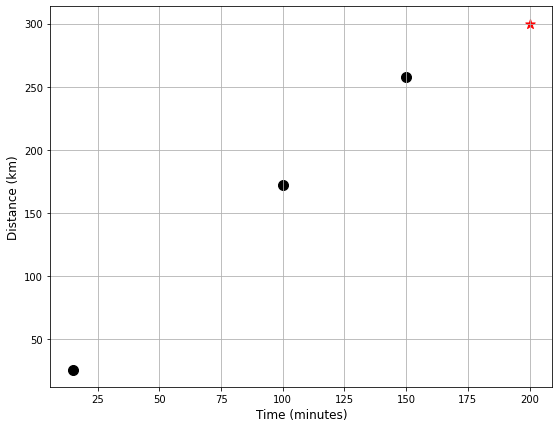
\includegraphics[width=0.55\linewidth]{interp1}
        \end{center}
      \end{figure}
  \end{itemize}
\end{frame}

\begin{frame}{Linear Interpolation}
  \begin{itemize}
  \item Since discount factors are available only at discrete times we need a procedure to determine the factors at \emph{every} time; the simplest technique is called \emph{interpolation}.
  \item \emph{Interpolation is a method to "determine" new points within a range of a discrete set of known data points.}
  \item Assume you are travelling by car at \emph{constant speed} (i.e. thetravelled distance is $s = v \cdot t$);
  \item if you plot the distances $s$ as a function of the time $t$ you get a line with slope $v$.
    \begin{figure}[h]
      \begin{center}
        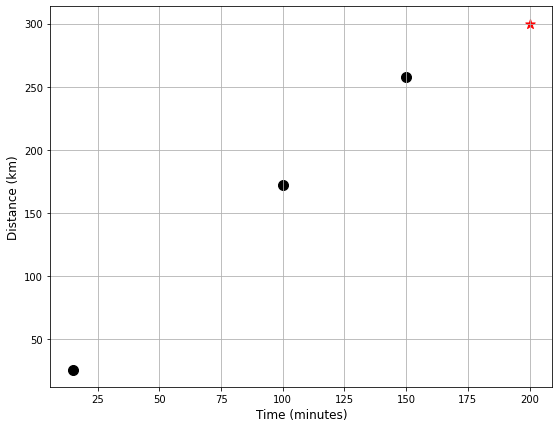
\includegraphics[width=0.55\linewidth]{interp1}
      \end{center}
    \end{figure}
  \end{itemize}
\end{frame}

\begin{frame}{Linear Interpolation}
  \begin{itemize}
  \item Imagine to have sampled few points of the function $s(t)$, we want to estimate it at $t_1 \leq \hat{t} \leq t_2$ which is not in our sample.
  \item To find $s(\hat{t})$ we can **linearly interpolate** between two sampled distances $s_1$ and $s_2$ (taken at $t_1$ and $t_2$):
    \begin{itemize}
    \item it works pretty much like a *weighted average* of the two sampled distances (full derivation in the notes);
    \item the closer point has more *influence* than the farther in the result.
    \end{itemize}
  \end{itemize}
\end{frame}

\begin{frame}{Linear Interpolation}
  Let's find the distance at $t = 60$ by interpolating between the two closer sampled points using the `python` function `numpy.interp`.
%  \begin{ipython}
%import numpy as np
%
%t = [15, 100, 150]
%s = [25.75, 171.7, 257.7]
%
%s_60 = np.interp(60, t, s)
%print (f"{s_60:.1f}")
%  \end{ipython}
%  \begin{ioutput}
%    103.0
%  \end{ioutput}
  \begin{block}{Always Interpret Critically your Results}
    In this case $t=60$ is almost in the middle of the interval $[t_1, t_2]$, so we expect to get a distance somehow in between $s_1$ and $s_2$, $s(t=60) \approx 100\;\textrm{km}$.
  \end{block}
  If we believe the relation between our variables stays the same (e.g. keep the same constant velocity in our trip), with the same mechanism we can alsp **extrapolate** values **outside** our initial sample.
  \begin{figure}[h]
    \begin{center}
      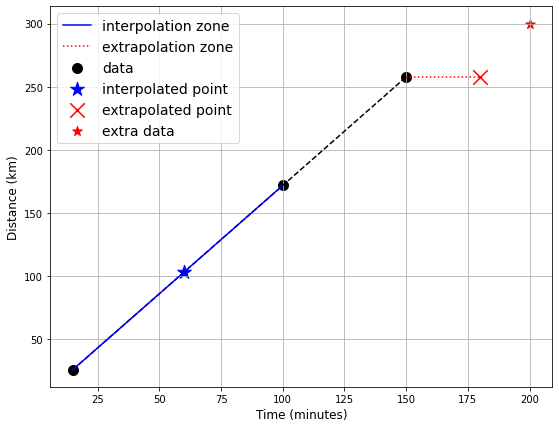
\includegraphics[width=0.55\linewidth]{interp2}
    \end{center}
  \end{figure}
  \texttt{numpy.interp} \emph{doesn't allow to extrapolate} returning always the closest measured value for points outside the interval.
\end{frame}

\begin{frame}{Log-linear Interpolation}
  \begin{itemize}
    \item When the function that we want to interpolate is an exponential we can fall back to the previous case by a simple variable transformation. 
      \begin{equation}
        \begin{gathered}
          p = \mathrm{exp}(v \cdot t) \\
          s = \mathrm{log}(p) = \mathrm{log}(\mathrm{exp}(v \cdot t)) = v \cdot t
        \end{gathered}
      \end{equation}

    \item So it is enough to use `numpy.interp` with the lists of $t$ and $\mathrm{log}(p)$ and **to exponentiate back at the end** to get the actual value of $p$.
  \end{itemize}
\end{frame}

\begin{frame}{Limitations of Linear Interpolation}
  \begin{itemize}
    \item Interpolation is just an \emph{approximation} and works well when either the function $s$ is linear or we are trying to interpolate between two points that are close enough that $s$ is \emph{almost} linear in that interval;
    \item intuitively the "curvier" the function the worse the approximation made with simple linear interpolation.
    \begin{figure}[h]
      \begin{center}
        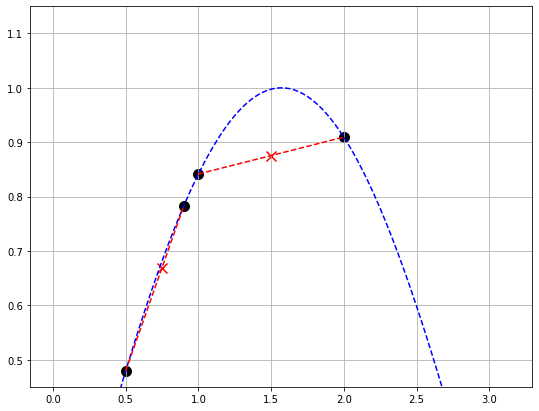
\includegraphics[width=0.55\linewidth]{interp3}
      \end{center}
    \end{figure}
  \end{itemize}
\end{frame}



* Let's put together what we have learnt so far (OOP and interpolation) by writing a `python` class which can handle **discount curves**.

<center>

![alt text](https://drive.google.com/uc?id=1qdOggwArqUmlPhHZZPXigMG3MSHALqVS)

</center> 

* **Attributes** (characteristic data of a discount curve):
  * a list of pillar dates (corresponding to the given discount factors), $t_0,...,t_{n-1}$
  * a list of discount factors, $D(t_0),...,D(t_{n-1})$

* **Methods** ("behaviour" of a discount curve):
  * one single method returning a discount factor at a given date (if necessary it must interpolate between existing factors);
  * since $D=e^{-r(T-t)}$ the method will use a log-linear interpolation to return the value we are looking for.

  $$d(t_i)=\log(D(t_i)) = \log(e^{-r(T-t_i)}) = -r(T-t_i) \;\;\textrm{where $i$ is such that}\;t_i \le t \le t_{i+1}$$

* **Note**: `numpy.interp` only accepts lists of numbers as arguments i.e. it doesn't automatically convert dates as numbers and doesn't know how to interpolate them. So you need to set an offset $t_0$ and convert each date into the number of days since $t_0$ before passing them to `numpy.interp`.

\begin{frame}{Forward Rates}
  \begin{itemize}
  \item A \emph{forward rate} is an interest rate applicable to a financial transaction that will take place in the future.
  \item It can be considered as the *market’s expectation for future prices* and can serve as an indicator of how it believes will perform.
  \item Contrary the \emph{spot rate} is used by buyers and sellers looking to make an immediate purchase or sale.
  \item To calculate the forward rates exploit no-arbitrage argument:
    \begin{equation}
      \begin{gathered}
        e^{r_1 (T_1-T_0)}e^{r_{1,2}(T_2 - T_1)} = e^{r_2 (T_2-T_0)} \implies e^{r_1 T_1 + r_{1,2}(T_2 - T_1)} = e^{r_2 T_2} \\
        r_1 T_1 + r_{1,2}(T_2 - T_1) = r_2 T_2 \implies r_{1,2} = \cfrac{r_2 T_2 - r_1 T_1 }{T_2 - T_1}
      \end{gathered}
    \end{equation}
  \end{itemize}
\end{frame}

### Forward Rate Class

* **Attributes**: 
  * pillar dates;
  * interest rates corresponding to the pillar dates.
* **Methods**:
  * a method to interpolate rate at a given date; 
  * a method to compute the forward rate relative to a time period.
\end{document}
